% SOURCE: perm_null_allcells/*.json :: gate_false_positive_rate (0/2000 all 22), n_perm=2000, cells.*.perm_p_one_sided (min plotted; GPT2_L36 min 0.83 off-scale, arrow-marked); gain for colouring: RG_gain_law_MERGED_REFIX20260730.json :: bundles.*.gain_median_absdrop_per_dose
% !TEX encoding = UTF-8 Unicode
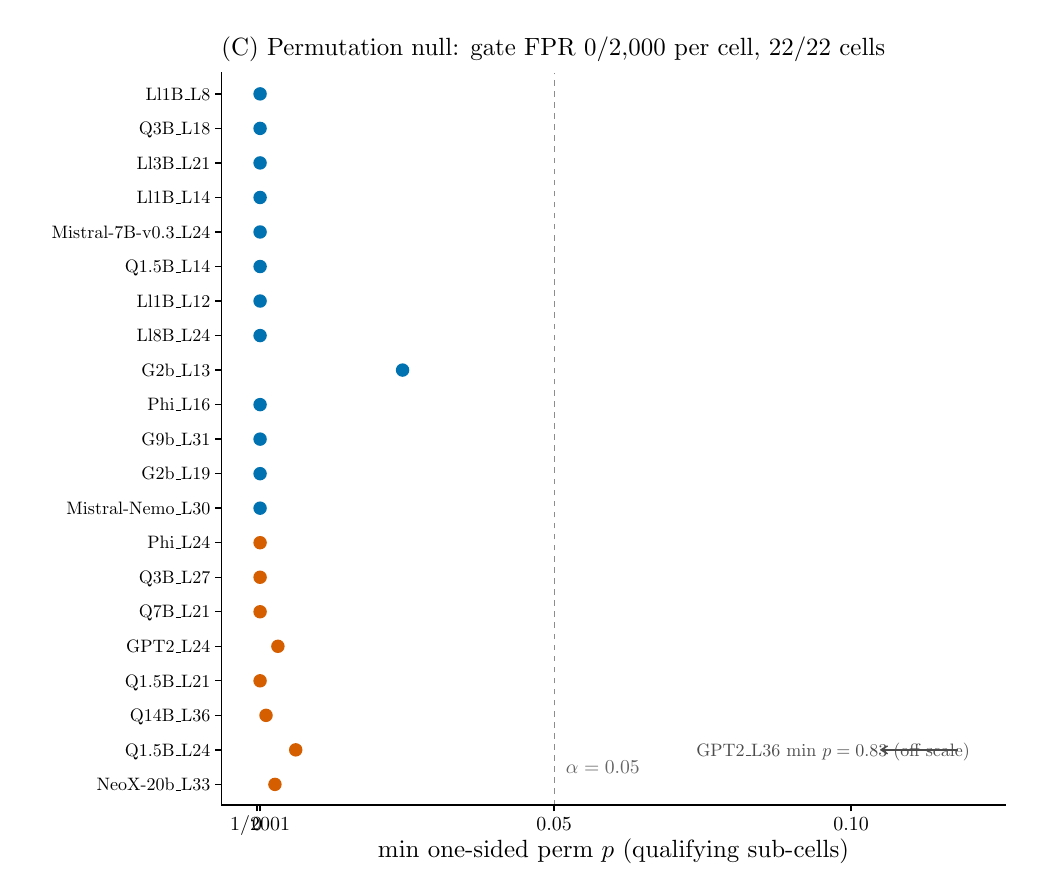
\begin{tikzpicture}[x=1pt,y=1pt]
\definecolor{fillColor}{RGB}{255,255,255}
\path[use as bounding box,fill=fillColor,fill opacity=0.00] (0,0) rectangle (361.35,303.53);
\begin{scope}
\path[clip] (  0.00,  0.00) rectangle (361.35,303.53);
\definecolor{drawColor}{RGB}{255,255,255}
\definecolor{fillColor}{RGB}{255,255,255}

\path[draw=drawColor,line width= 0.5pt,line join=round,line cap=round,fill=fillColor] (  0.00,  0.00) rectangle (361.35,303.53);
\end{scope}
\begin{scope}
\path[clip] ( 70.03, 22.61) rectangle (353.35,287.09);
\definecolor{fillColor}{RGB}{255,255,255}

\path[fill=fillColor] ( 70.03, 22.61) rectangle (353.35,287.09);
\definecolor{drawColor}{gray}{0.55}

\path[draw=drawColor,line width= 0.4pt,dash pattern=on 2pt off 2pt ,line join=round] (190.23, 22.61) -- (190.23,287.09);
\definecolor{fillColor}{RGB}{0,114,178}

\path[fill=fillColor] ( 83.98,279.60) circle (  2.43);

\path[fill=fillColor] ( 83.98,267.13) circle (  2.43);

\path[fill=fillColor] ( 83.98,254.65) circle (  2.43);

\path[fill=fillColor] ( 83.98,242.17) circle (  2.43);

\path[fill=fillColor] ( 83.98,229.70) circle (  2.43);

\path[fill=fillColor] ( 83.98,217.22) circle (  2.43);

\path[fill=fillColor] ( 83.98,204.75) circle (  2.43);

\path[fill=fillColor] ( 83.98,192.27) circle (  2.43);

\path[fill=fillColor] (135.47,179.80) circle (  2.43);

\path[fill=fillColor] ( 83.98,167.32) circle (  2.43);

\path[fill=fillColor] ( 83.98,154.85) circle (  2.43);

\path[fill=fillColor] ( 83.98,142.37) circle (  2.43);

\path[fill=fillColor] ( 83.98,129.90) circle (  2.43);
\definecolor{fillColor}{RGB}{213,94,0}

\path[fill=fillColor] ( 83.98,117.42) circle (  2.43);

\path[fill=fillColor] ( 83.98,104.94) circle (  2.43);

\path[fill=fillColor] ( 83.98, 92.47) circle (  2.43);

\path[fill=fillColor] ( 90.42, 79.99) circle (  2.43);

\path[fill=fillColor] ( 83.98, 67.52) circle (  2.43);

\path[fill=fillColor] ( 86.13, 55.04) circle (  2.43);

\path[fill=fillColor] ( 96.86, 42.57) circle (  2.43);

\path[fill=fillColor] ( 89.35, 30.09) circle (  2.43);
\definecolor{drawColor}{gray}{0.40}

\node[text=drawColor,anchor=base west,inner sep=0pt, outer sep=0pt, scale=  0.71] at (194.52, 33.88) {$\alpha = 0.05$};
\definecolor{drawColor}{gray}{0.30}

\path[draw=drawColor,line width= 0.5pt,line join=round] (336.18, 42.57) -- (308.28, 42.57);

\path[draw=drawColor,line width= 0.5pt,line join=round] (310.74, 43.99) --
	(308.28, 42.57) --
	(310.74, 41.14);

\node[text=drawColor,anchor=base east,inner sep=0pt, outer sep=0pt, scale=  0.65] at (340.47, 40.31) {GPT2\_L36 min $p = 0.83$ (off scale)};
\end{scope}
\begin{scope}
\path[clip] (  0.00,  0.00) rectangle (361.35,303.53);
\definecolor{drawColor}{RGB}{0,0,0}

\path[draw=drawColor,line width= 0.5pt,line join=round,line cap=rect] ( 70.03, 22.61) --
	( 70.03,287.09);
\end{scope}
\begin{scope}
\path[clip] (  0.00,  0.00) rectangle (361.35,303.53);
\definecolor{drawColor}{RGB}{0,0,0}

\node[text=drawColor,anchor=base east,inner sep=0pt, outer sep=0pt, scale=  0.65] at ( 65.98, 27.85) {NeoX-20b\_L33};

\node[text=drawColor,anchor=base east,inner sep=0pt, outer sep=0pt, scale=  0.65] at ( 65.98, 40.33) {Q1.5B\_L24};

\node[text=drawColor,anchor=base east,inner sep=0pt, outer sep=0pt, scale=  0.65] at ( 65.98, 52.80) {Q14B\_L36};

\node[text=drawColor,anchor=base east,inner sep=0pt, outer sep=0pt, scale=  0.65] at ( 65.98, 65.28) {Q1.5B\_L21};

\node[text=drawColor,anchor=base east,inner sep=0pt, outer sep=0pt, scale=  0.65] at ( 65.98, 77.76) {GPT2\_L24};

\node[text=drawColor,anchor=base east,inner sep=0pt, outer sep=0pt, scale=  0.65] at ( 65.98, 90.23) {Q7B\_L21};

\node[text=drawColor,anchor=base east,inner sep=0pt, outer sep=0pt, scale=  0.65] at ( 65.98,102.71) {Q3B\_L27};

\node[text=drawColor,anchor=base east,inner sep=0pt, outer sep=0pt, scale=  0.65] at ( 65.98,115.18) {Phi\_L24};

\node[text=drawColor,anchor=base east,inner sep=0pt, outer sep=0pt, scale=  0.65] at ( 65.98,127.66) {Mistral-Nemo\_L30};

\node[text=drawColor,anchor=base east,inner sep=0pt, outer sep=0pt, scale=  0.65] at ( 65.98,140.13) {G2b\_L19};

\node[text=drawColor,anchor=base east,inner sep=0pt, outer sep=0pt, scale=  0.65] at ( 65.98,152.61) {G9b\_L31};

\node[text=drawColor,anchor=base east,inner sep=0pt, outer sep=0pt, scale=  0.65] at ( 65.98,165.08) {Phi\_L16};

\node[text=drawColor,anchor=base east,inner sep=0pt, outer sep=0pt, scale=  0.65] at ( 65.98,177.56) {G2b\_L13};

\node[text=drawColor,anchor=base east,inner sep=0pt, outer sep=0pt, scale=  0.65] at ( 65.98,190.03) {Ll8B\_L24};

\node[text=drawColor,anchor=base east,inner sep=0pt, outer sep=0pt, scale=  0.65] at ( 65.98,202.51) {Ll1B\_L12};

\node[text=drawColor,anchor=base east,inner sep=0pt, outer sep=0pt, scale=  0.65] at ( 65.98,214.99) {Q1.5B\_L14};

\node[text=drawColor,anchor=base east,inner sep=0pt, outer sep=0pt, scale=  0.65] at ( 65.98,227.46) {Mistral-7B-v0.3\_L24};

\node[text=drawColor,anchor=base east,inner sep=0pt, outer sep=0pt, scale=  0.65] at ( 65.98,239.94) {Ll1B\_L14};

\node[text=drawColor,anchor=base east,inner sep=0pt, outer sep=0pt, scale=  0.65] at ( 65.98,252.41) {Ll3B\_L21};

\node[text=drawColor,anchor=base east,inner sep=0pt, outer sep=0pt, scale=  0.65] at ( 65.98,264.89) {Q3B\_L18};

\node[text=drawColor,anchor=base east,inner sep=0pt, outer sep=0pt, scale=  0.65] at ( 65.98,277.36) {Ll1B\_L8};
\end{scope}
\begin{scope}
\path[clip] (  0.00,  0.00) rectangle (361.35,303.53);
\definecolor{drawColor}{RGB}{0,0,0}

\path[draw=drawColor,line width= 0.5pt,line join=round] ( 67.78, 30.09) --
	( 70.03, 30.09);

\path[draw=drawColor,line width= 0.5pt,line join=round] ( 67.78, 42.57) --
	( 70.03, 42.57);

\path[draw=drawColor,line width= 0.5pt,line join=round] ( 67.78, 55.04) --
	( 70.03, 55.04);

\path[draw=drawColor,line width= 0.5pt,line join=round] ( 67.78, 67.52) --
	( 70.03, 67.52);

\path[draw=drawColor,line width= 0.5pt,line join=round] ( 67.78, 79.99) --
	( 70.03, 79.99);

\path[draw=drawColor,line width= 0.5pt,line join=round] ( 67.78, 92.47) --
	( 70.03, 92.47);

\path[draw=drawColor,line width= 0.5pt,line join=round] ( 67.78,104.94) --
	( 70.03,104.94);

\path[draw=drawColor,line width= 0.5pt,line join=round] ( 67.78,117.42) --
	( 70.03,117.42);

\path[draw=drawColor,line width= 0.5pt,line join=round] ( 67.78,129.90) --
	( 70.03,129.90);

\path[draw=drawColor,line width= 0.5pt,line join=round] ( 67.78,142.37) --
	( 70.03,142.37);

\path[draw=drawColor,line width= 0.5pt,line join=round] ( 67.78,154.85) --
	( 70.03,154.85);

\path[draw=drawColor,line width= 0.5pt,line join=round] ( 67.78,167.32) --
	( 70.03,167.32);

\path[draw=drawColor,line width= 0.5pt,line join=round] ( 67.78,179.80) --
	( 70.03,179.80);

\path[draw=drawColor,line width= 0.5pt,line join=round] ( 67.78,192.27) --
	( 70.03,192.27);

\path[draw=drawColor,line width= 0.5pt,line join=round] ( 67.78,204.75) --
	( 70.03,204.75);

\path[draw=drawColor,line width= 0.5pt,line join=round] ( 67.78,217.22) --
	( 70.03,217.22);

\path[draw=drawColor,line width= 0.5pt,line join=round] ( 67.78,229.70) --
	( 70.03,229.70);

\path[draw=drawColor,line width= 0.5pt,line join=round] ( 67.78,242.17) --
	( 70.03,242.17);

\path[draw=drawColor,line width= 0.5pt,line join=round] ( 67.78,254.65) --
	( 70.03,254.65);

\path[draw=drawColor,line width= 0.5pt,line join=round] ( 67.78,267.13) --
	( 70.03,267.13);

\path[draw=drawColor,line width= 0.5pt,line join=round] ( 67.78,279.60) --
	( 70.03,279.60);
\end{scope}
\begin{scope}
\path[clip] (  0.00,  0.00) rectangle (361.35,303.53);
\definecolor{drawColor}{RGB}{0,0,0}

\path[draw=drawColor,line width= 0.5pt,line join=round,line cap=rect] ( 70.03, 22.61) --
	(353.35, 22.61);
\end{scope}
\begin{scope}
\path[clip] (  0.00,  0.00) rectangle (361.35,303.53);
\definecolor{drawColor}{RGB}{0,0,0}

\path[draw=drawColor,line width= 0.5pt,line join=round] ( 82.91, 20.36) --
	( 82.91, 22.61);

\path[draw=drawColor,line width= 0.5pt,line join=round] ( 83.98, 20.36) --
	( 83.98, 22.61);

\path[draw=drawColor,line width= 0.5pt,line join=round] (190.23, 20.36) --
	(190.23, 22.61);

\path[draw=drawColor,line width= 0.5pt,line join=round] (297.55, 20.36) --
	(297.55, 22.61);
\end{scope}
\begin{scope}
\path[clip] (  0.00,  0.00) rectangle (361.35,303.53);
\definecolor{drawColor}{RGB}{0,0,0}

\node[text=drawColor,anchor=base,inner sep=0pt, outer sep=0pt, scale=  0.72] at ( 82.91, 13.60) {0};

\node[text=drawColor,anchor=base,inner sep=0pt, outer sep=0pt, scale=  0.72] at ( 83.98, 13.60) {$1/2001$};

\node[text=drawColor,anchor=base,inner sep=0pt, outer sep=0pt, scale=  0.72] at (190.23, 13.60) {0.05};

\node[text=drawColor,anchor=base,inner sep=0pt, outer sep=0pt, scale=  0.72] at (297.55, 13.60) {0.10};
\end{scope}
\begin{scope}
\path[clip] (  0.00,  0.00) rectangle (361.35,303.53);
\definecolor{drawColor}{RGB}{0,0,0}

\node[text=drawColor,anchor=base,inner sep=0pt, outer sep=0pt, scale=  0.90] at (211.69,  3.75) {min one-sided perm $p$ (qualifying sub-cells)};
\end{scope}
\begin{scope}
\path[clip] (  0.00,  0.00) rectangle (361.35,303.53);
\definecolor{drawColor}{RGB}{0,0,0}

\node[text=drawColor,anchor=base west,inner sep=0pt, outer sep=0pt, scale=  0.90] at ( 70.03,293.34) {(C) Permutation null: gate FPR 0/2{,}000 per cell, 22/22 cells};
\end{scope}
\end{tikzpicture}
